\documentclass[border=3pt]{standalone}
% Shared preamble for standalone TikZ figures (colors match the slide theme).
\usepackage[T1]{fontenc}
\IfFileExists{sourcesanspro.sty}{\usepackage[default]{sourcesanspro}}{\usepackage[scaled=0.92]{helvet}\renewcommand{\familydefault}{\sfdefault}}
\usepackage{xcolor,tikz}
\usetikzlibrary{arrows.meta,positioning,calc,shapes.geometric,decorations.pathmorphing,decorations.pathreplacing,backgrounds,fit}
\definecolor{fsNavy}{HTML}{1B365D}
\definecolor{fsAccent}{HTML}{C8102E}
\definecolor{fsGold}{HTML}{D39B1E}
\definecolor{fsTeal}{HTML}{1F7A8C}
\definecolor{fsGreen}{HTML}{3A7D44}
\definecolor{fsGray}{HTML}{5B6770}
\definecolor{fsLight}{HTML}{EEF2F6}
\tikzset{
  molbox/.style={draw=black!55,rounded corners=3pt,line width=0.6pt,
                 minimum height=7mm,font=\small\bfseries,inner xsep=3mm},
  site/.style={circle,draw=black!55,fill=white,inner sep=0pt,minimum size=4mm,
               font=\tiny\bfseries,line width=0.5pt},
  psite/.style={site,fill=fsAccent,text=white},
  bond/.style={line width=1.3pt,black!70},
  callout/.style={font=\scriptsize,text=fsGray,align=left},
  pointer/.style={-{Stealth[length=1.6mm]},fsGray,line width=0.5pt},
}
\newcommand{\code}[1]{{\ttfamily #1}}

\begin{document}
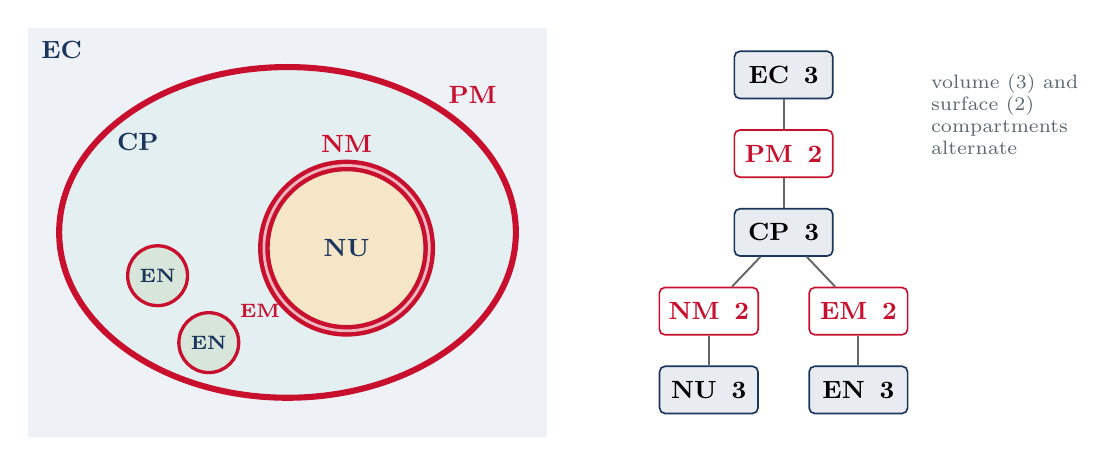
\begin{tikzpicture}[x=1cm,y=1cm,
    vol/.style={draw=none,font=\small\bfseries},
    surf/.style={font=\small\bfseries,text=fsAccent},
    tnode/.style={rounded corners=2pt,minimum width=1.25cm,minimum height=6mm,font=\small\bfseries,line width=0.6pt},
    tvol/.style={tnode,draw=fsNavy,fill=fsNavy!10},
    tsurf/.style={tnode,draw=fsAccent,fill=white,text=fsAccent},
    tedge/.style={line width=0.7pt,black!60}]
  % ---- cell sketch ----
  \fill[fsLight] (-3.3,-2.6) rectangle (3.3,2.6);
  \node[vol,anchor=north west,text=fsNavy] at (-3.25,2.55) {EC};
  \draw[fsAccent,line width=2.2pt,fill=fsTeal!12] (0,0) ellipse (2.9 and 2.1);
  \node[surf] at (2.35,1.75) {PM};
  \node[vol,text=fsNavy] at (-1.9,1.15) {CP};
  % nucleus
  \draw[fsAccent,line width=1.6pt,double=fsAccent!30,double distance=1pt,fill=fsGold!25] (0.75,-0.2) circle (1.05);
  \node[vol,text=fsNavy] at (0.75,-0.2) {NU};
  \node[surf] at (0.75,1.12) {NM};
  % endosomes
  \foreach \x/\y in {-1.65/-0.55,-1.0/-1.4} {
    \draw[fsAccent,line width=1.2pt,fill=fsGreen!20] (\x,\y) circle (0.38);
  }
  \node[vol,text=fsNavy,font=\scriptsize\bfseries] at (-1.65,-0.55) {EN};
  \node[vol,text=fsNavy,font=\scriptsize\bfseries] at (-1.0,-1.4) {EN};
  \node[surf,font=\scriptsize\bfseries] at (-0.35,-1.0) {EM};
  % ---- tree ----
  \begin{scope}[xshift=6.3cm,yshift=2.0cm]
    \node[tvol]  (EC) at (0,0)     {EC \,3};
    \node[tsurf] (PM) at (0,-1)    {PM \,2};
    \node[tvol]  (CP) at (0,-2)    {CP \,3};
    \node[tsurf] (NM) at (-0.95,-3) {NM \,2};
    \node[tvol]  (NU) at (-0.95,-4) {NU \,3};
    \node[tsurf] (EM) at (0.95,-3)  {EM \,2};
    \node[tvol]  (EN) at (0.95,-4)  {EN \,3};
    \draw[tedge] (EC)--(PM); \draw[tedge] (PM)--(CP);
    \draw[tedge] (CP)--(NM); \draw[tedge] (CP)--(EM);
    \draw[tedge] (NM)--(NU); \draw[tedge] (EM)--(EN);
    \node[callout,anchor=west] at (1.75,-0.5) {volume (3) and\\surface (2)\\compartments\\alternate};
  \end{scope}
\end{tikzpicture}
\end{document}
